\section{Requisitos}
\label{sec:requisitos}
\subsection{Requisitos Funcionais}

\begin{itemize}
\item Armazenar garrafas recicláveis.
\item Bonificar usuário por entrega de garrafas.
\item Armazenamento separado pelos tipos de materiais de garrafas.
\item Triturar as garrafas de plástico.
\item Validar o tipo de objeto a ser inserido na máquina.
\item A alimentação energética será diretamente pela rede elétrica.
\item Deverá haver a interação de reconhecimento direto entre máquina e usuário.
\item Manter dados do usuário.
\item Projeto de estrutura que comporte aparatos tecnológicos.
\item Projeto de estrutura que comporte o motor, o separador, triturador e compartimentos de armazenagem.

\end{itemize}

\subsection{Requisitos Não Funcionais}

\begin{itemize}
\item Haverá sistema de segurança de desligamento do motor.
\item Armazenar as garrafas de vidro de forma intacta.
\item O sistema da máquina deve guardar os dados em um banco em nuvem.
\item A máquina deve atender à normas legais.
\item A máquina terá seu uso liberado após a identificação do usuário.
\item Não deve ser exposto nenhum dado privado do usuário de forma livre.
\item A estrutura do triturador deve ser extremamente fechado a qualquer contato do usuário. 

\end{itemize}

\section{Estudo da Viabilidade do Projeto}

\section{Escopo}
\subsection{Definição do Escopo}

\subsection{Processo de Formalização de Aprovação}
    Este processo tem por objetivo regular todas as entregas feitas durante o desenvolvimento do sistema.

    Segue o processo e suas respectivas atividades descritas.

\begin{figure}[!ht]
	\centering
		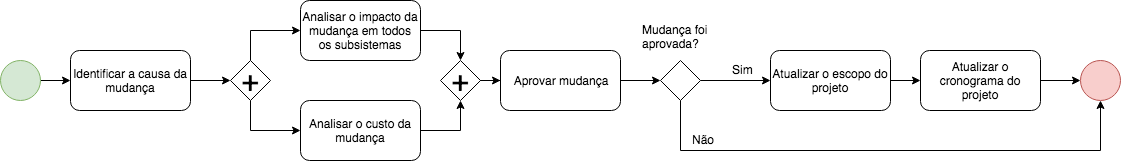
\includegraphics{figuras/mudanca}
	\caption{Processo de Gerenciamento de Mudança.}
\end{figure}

\begin{itemize}
    \item \textbf{Testar entrega}
        Nesta atividade, deve-se garantir que o que foi desenvolvido está pronto para uso e integração com o resto do sistema, bem como se não apresenta falhas na possibilidade de uso extremo do que foi desenvolvido.

    \item \textbf{Processo de Gerenciamento de Mudança}
        Caso o que foi desenvolvido não esteja de acordo com o que foi previamente acordado nos requisitos do projeto, descritos no começo dessa seção, a mudança deve ser passada por um Processo de Gerenciamento de Mudança antes que possa ser aprovado. O processo em si é melhor descrito na próxima seção.

    \item \textbf{Aprovar entrega}
        Uma vez que a entrega está testada e de acordo com os requisitos do projeto ela pode ser dita como entregue.
\end{itemize}

\subsection{Processo de Gerenciamento de Mudança}
    Sempre que for necessário que mudanças ocorram dentro do sistema, primeiro deve ser executado um processo de gerenciamento de mudança para garantir que a mesma não terá um impacto negativo sobre o projeto.

    O processo, bem como a descrição de suas atividades, estão disponíveis abaixo.

\begin{figure}[!ht]
	\centering
		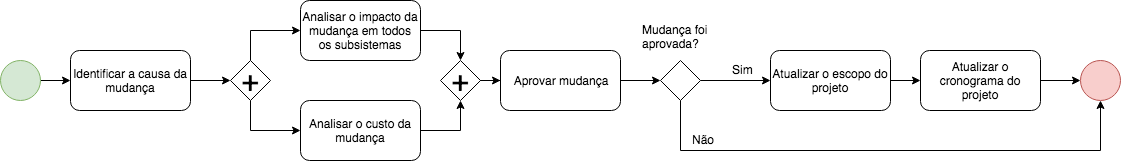
\includegraphics{figuras/mudanca}
	\caption{Processo de Gerenciamento de Mudança.}
\end{figure}

\begin{itemize}

    O processo de gerenciamento de mudança envole as seguintes atividades:

    \item \textbf{Identificar a causa da mudança}
        Nesta atividade deve ser identificada a mudança a ser executa e a razão de tal mudança, afim de facilitar as próximas atividades do processo.

    \item \textbf{Analisar o impacto da mudança em todos os subsistemas}
        Uma vez identificada a causa da mudança, a equipe deverá analisar como a mudança irá afetar todos os subsistemas do projeto. Essa atividade deverá resultar na identificação de tudo o que deve ser alterado em cada subsistema, bem como em sua respectiva análise.

    \item \textbf{Analisar o custo da mudança}
        Nesta atividade a equipe deve analisar o custo que a mudança trará ao projeto, tanto a nível financeiro como a nível de tempo restante para desenvolvimento do projeto.

    \item\textbf{Aprovar mudança}
        Com base nas análises de custo e impacto feitas, a equipe deve decidir se a mesma será aprovada caso não haja prejuízo.

    \item \textbf{Atualizar o escopo do projeto}
        Todas as mudanças identificadas na atividade de Analisar o impacto da mudança em todos os subsistemas devem ser incorporadas ao escopo.

    \item \textbf{Atualizar o cronograma do projeto}
        Para que o prazo do projeto seja respeitado, o cronograma deve passar a englobar as mudanças feitas no escopo na atividade previamente descrita.

\end{itemize}

\section{Análise Crítica de Projeto e Desenvolvimento}

\subsection{Processo de Gerenciamento dos Riscos}
    Este processo tem por objetivo controlar e minimizar os eventuais impedimentos que venham a acontecer durante o desenvolimento do projeto.

\section{Recursos Humanos}
\subsection{Papéis e responsabilidades}

\subsection{Organograma}    

    
    

